% \section{Quantum Perceptron with Quantum Activation Function}
우리는 양자 머신러닝의 큰 진입장벽 중 하나가 비선형성의 구현이라는 것을 이전 장에서 발견했다.
양자 알고리즘의 각 step, 즉 각 게이트를 통과하는 프로세스 하나하나는 본질적으로 각 게이트에 대응되는 행렬을 벡터에 곱해 주는 작업이다.
행렬곱은 선형 연산이다. 즉 양자 알고리즘은 선형 연산이다. 결국 양자 알고리즘으로 완전한 비선형성의 구현이 불가능하다는 결론에 이르게 된다. 이것은 우리의 과제에 있어 큰 장벽이다.
인공지능, 그중에서도 MLP(Multi Layer Perceptron)는 행렬 연산의 반복으로 구성되는데, 행렬 연산의 차원을 높이기 위해 각 Layer 사이에 비선형 연산을 추가하는 것이 필수적이기 때문이다.
해당 문제의 해결이 선행되기 전까지 MLP를 양자 알고리즘만으로 완전히 구현하는 것은 불가능하다는 것을 어렵지 않게 떠올릴 수 있다.
그렇기에 고전 알고리즘과 양자 알고리즘을 적절히 섞어 사용하는 Hybrid Algorithm이라는 대안이 존재하나, 양자 알고리즘만으로 머신 러닝의 과정을 모두 구현하겠다는 시도는 분명 학술적으로 그 가치가 충분하다.

우리는 상기한 비선형성 구현 문제의 해결 방법 하나를 제시한 논문을 발견하였다.
해당 논문에는 단층 퍼셉트론의 연산 프로세스를 양자 회로로 구현하는 방법이 제시되어 있다.
단층 퍼셉트론은 크게 \(N_{in} \times 1\) 크기의 input vector \(\vec{x}\),
\(\vec{x}\)의 각 성분과 곱해지게 될 가중치 값이 저장되어 있는 \(N_{in} \times 1\) 크기의 weight vector \(\vec{w}\),
스칼라 값인 bias \(b\), 그리고 비선형성을 위한 활성화 함수(Activation Function, AF) \(f\)로 구성되어,
\(\vec{x}\)가 input으로 주어지면 \(f(\vec{w}\cdot\vec{x}+b)\)의 값을 내놓는다.
해당 논문은 \(\vec{w}\cdot\vec{x}+b\)의 계산뿐만 아니라, \(f(\vec{w}\cdot\vec{x}+b)\)의 계산 또한 양자 알고리즘으로 구현한다.
\(f\) 함수 자체는 사용할 수 없으나, 양자 회로를 잘 구성하여 \(f(\vec{w}\cdot\vec{x}+b)\)의 값을 근사적으로 구하는 방법론을 제시한 것이다.

우리는 해당 논문을 이번 연구의 중심 축으로 결정하였다.
우리는 해당 논문을 이해하고, 수학적 과정을 코드로 구현하여 직접 확인해 보았다.
또한 논문에서는 제대로 논의하고 있지 않은 부분인 MLP의 양자적 구현을 고민하던 중, 우리는 매우 효율적인 Multiperceptron의 양자 알고리즘을 구현하는 데에 성공하였고, 이를 코드로 구현하여 잘 작동함을 확인하였다.

이번 장은 해당 논문에 대한 우리의 심도 깊은 이해와 구현, 그리고 우리가 발전시킨 부분에 대해 서술되어 있다.
3.1장에서는 \(f(\vec{w}\cdot\vec{x}+b)\)를 양자 알고리즘으로 구현하는 과정을 따라가고, 그 과정을 직접 코드로 구현해 본 과정을 공유한다.
이후 3.2장에서는 우리의 독창적이고 효율적인 Multiperceptron의 구현 아이디어에 대해 설명한다.

\section{Imparting Nonlinearity for Quantum Perceptron}

\subsection{Summarization of the Notations}

이번 Section은 앞으로의 내용을 잘 이해하기 위해 기호들이나 용어의 의미를 미리 정리하고 가기 위한 장이다.

앞으로 qubit의 개수를 표기하는 영어 소문자에 대해, 대문자 표기는 그 qubit에 대응되는 힐베르트 공간의 차원을 나타낸다.
즉 qubit 개수가 n인 경우, N = \(2^n\)이다.

임의의 1개 qubit과 대응되는 2차원 힐베르트 공간 \(\mathcal{H}\)에 대하여, register q의 n개의 qubit과 대응되는 \(2^n\)차원 힐베르트 공간을 \(\mathcal{H}_q^{\otimes n} \equiv \mathcal{H}_{q_{n-1}} \otimes \mathcal{H}_{q_{n-2}} \otimes \dots \otimes \mathcal{H}_{q_{0}}\) 라고 한다.
이때 register는 qubit이 저장되어 있는 공간의 이름을 말한다. 간단하게 이해하면 qubit의 집합이라고 생각하면 된다.
\(\mathcal{H}\)의 computational basis가 \(\{ \ket{0}, \ket{1} \}\)임을 일전에 이야기했다. 그렇기에 \(\mathcal{H}_q^{\otimes n}\)의 computational basis는 \(\{ \ket{s_{n-1}s_{n-2}\dots s_0} : s_k \in \{0,1\}, k = 0,1,\dots , n-1\}\)의 이진수 형태로 나타내어지고, 각 원소는 이를 십진수 형태로 변환한 \(\{ \ket{i}, i \in \{0,1,\dots,2^n-1\} \} \)의 형태로 나타낼 수도 있다.
예컨대, \(\ket{N-1} \equiv \ket{2^n-1} \equiv \ket{111\dots 1} \equiv \ket{1}^{\otimes n}\)가 된다.

n개의 qubit으로 구성된 register q에 적용되는 연산 U를 표기하는 방법은, U가 separable인지 아닌지에 따라 나뉜다.
sperable이 아닌 경우에는 U가 q에 가해지는 연산임을 나타내기 위해 \(U_q\)라고 작성하거나, 아니면 단순히 U라고 적는다.
한편, U가 one-qubit transformation \(U_{q_j}\)들의 텐서곱으로 나타내어지는, 즉 separable인 경우에는 U를 \(U_q^{\otimes n} \equiv U_{q_{n-1}} \otimes U_{q_{n-2}} \otimes \dots \otimes U_{q_{0}}\)라고 적는다.

n개의 qubit으로 구성된 register q, d개의 qubit으로 구성된 register a를 생각하자. 두 레지스터는 N+D차원 Hibert Space로 합쳐질 수 있다. 이 합쳐진 Space를 \(\mathcal{H}_a^{\otimes d} \otimes \mathcal{H}_q^{\otimes n}\)로 작성한다. 이때 이 Space의 computational basis는 \(\{ \ket{i}_a \ket{j}_q : i = 0,\dots,D-1, j = 0,\dots,N-1\}\)이다.
간결함을 위해, 연산 O가 만약 둘 중 하나의 register에서만 작동하는 경우에 \(\mathbb{1}_a \otimes O_q, O_a \otimes \mathbb{1}_q\)를 각각 \(O_q, O_a\)로 간단하게 나타낸다. 이때 \(\mathbb{1}_a = I_{2^d}\)를 의미한다.
특히, \(\ket{i}\bra{i}_q \equiv \mathbb{1}_a \otimes \ket{i}_q {_q}\bra{i}\)는 register q의 \(\ket{i}\) state로의 D차원 projection을 나타낸다.

마지막으로, controlled gate(특정 qubit의 상태에 따라 연산의 작동 여부가 결정되는 게이트)를 나타내기 위해 사용하는 표기들을 정리해 보자. \(C_{q_i}U_{q_j}\)라는 표기는 \(q_i\) qubit의 state가 \(\ket{1}\)일 때 \(q_j\) qubit에 연산 U를 가하겠다는 의미이다.
이와 반대로 \(\bar{C_{q_i}}U_{q_j}\)은 \(q_i\) qubit의 state가 \(\ket{0}\)일 때 \(q_j\) qubit에 연산 U를 가하겠다는 의미이다.
즉 \(\bar{C_{q_i}}U_{q_j}\)은 \(X_{q_i}C_{q_i}U_{q_j}X_{q_i}\)와 동일한 연산이다. (X: Pauli-X gate)
만약 d개의 qubit으로 구성된 register a의 모든 qubit을 control qubit으로 사용하는 경우에는 \(C_a^dU_{q_j}\)라는 표기를 사용한다.

\subsection{Implementation of \(\vec{w}\cdot\vec{x}+b\)}

단일 퍼셉트론의 구현을 위해 n+d개의 qubit이 필요하다. n개의 qubit은 q register에, d개의 qubit은 a register에 들어 있다. input vector \(\vec{x}\)의 크기는 \(N_{in}\)으로 쓴다.
우선은 각 input값을 scaling하여 각 성분을 -1과 1 사이의 값으로 고정시키는 것으로 시작한다.
즉, \(\vec{w} \in [-1,1]^{N_{in}}, \vec{x} \in [-1,1]^{N_{in}}, b \in [-1,1]\)이 주어졌을 때, \(\vec{w}\cdot\vec{x}+b\)의 값을 계산하는 양자 회로의 구성 과정을 따라가 보겠다.
이 장과 그 다음 장은 본질적으로 우리의 논문 탐독 과정을 따라가기 위한 것이기에, 논문의 주요 Theorem을 직접 인용하고, 그 의미와 증명의 흐름을 간단하게 서술하는 것으로 구성하였다. 논문 원문에는 증명 전체가 서술되어 있으므로,
자세한 이해를 원한다면 Reference를 참고할 수 있다.

%\begin{lemma}
%    \(\vec{x}, \vec{w}, b\) 가 주어졌을 때, \(\displaystyle \bra{N-1}U_z(\vec{x},\vec{w},b)\ket{0} = \frac{\vec{x}\cdot \vec{w}+b}{N_{in}+1} \equiv z\) 를 만족하는 Unitary transformation \(U_z(\vec{x},\vec{w},b)\) 의 역할을 하는 양자 회로를 만들 수 있다.
%\end{lemma}

\begin{lemma}

    Given two vectors $\vec{x}, \vec{w} \in [-1, 1]^{N_{\text{in}}}$ and a number $b \in [-1, 1]$, and given a register of $n$ qubits such that $N = 2^n \geq N_{\text{in}} + 3$, then there exists a quantum circuit realizing a unitary transformation $U_z(\vec{x}, \vec{w}, b)$ such that
\[
\langle N - 1 | U_z(\vec{x}, \vec{w}, b) | 0 \rangle = \frac{\vec{w} \cdot \vec{x} + b}{N_{\text{in}} + 1} \equiv z
\]
where $\ket{0} \equiv \ket{0}^{\otimes n}$ and $\ket{N-1} \equiv \ket{1}^{\otimes n}$.

\end{lemma}

우선, \(\vec{w}\cdot \vec{x} + b\)의 구현을 위한 양자 회로의 구성 요소 중 필수적인, \(U_z(\vec{x},\vec{w},b)\) 부분의 기능을 구현하기 위한 Lemma가 제시된다.
대략적인 증명의 흐름은 다음과 같다.

\begin{pf}(sketch)

Lemma에서 \(\ket{0}, \ket{N-1}\)은 각각 \(\ket{0}^{\otimes n}, \ket{1}^{\otimes n}\)임을 기억하자.
\(\vec{v}_x = (\vec{x},1,A_x,\vec{0}), \vec{v}_{w,b} = (\vec{w},b,\vec{0},A_{w,b})\) 를 만들자.
이때 두 벡터는 \(n = \lceil\log_2{N_{in}+3}\rceil\)에 대해 \(N = 2^n\)의 크기를 가진다. 벡터의 성분으로 들어 있는 0의 개수는 N과 \(N_{in}\)값에 따라 결정된다.
또한, 두 벡터는 \(|\vec{v}_x| = |\vec{v}_{w,b}| = \sqrt{N_{in}+1}\)를 만족해야만 한다. \(A_x, A_{w,b}\)의 값은 해당 규칙에 맞게 결정해 주면 된다.
그러면 \(\vec{v}_{w,b}^T\vec{v}_{x} = \vec{w}\cdot\vec{x}+b \in [-N_{in}-1, N_{in}+1]\)이 자연스럽게 도출된다.

%두 개의 state \(\ket{\psi_{x}},\ket{\psi_{w,b}}\)를 각각 \(\ket{\psi_{x}} = \sum_{i=0}^{N-1}\frac{v_{x,i}}{\sqrt{N_{in}+1}}\ket{i}, \ket{\psi_{w,b}} = \sum_{i=0}^{N-1}\frac{v_{w,b,i}}{\sqrt{N_{in}+1}}\ket{i}\)라 정의하자.
%그러면 \(\bra{\psi_x}\ket{\psi_{w,b}} = \frac{\vec{w}\cdot\vec{x}+b}{N_{in}+1} \equiv z\)가 성립한다.

위에서 만든 두 벡터 \(\vec{v}_x, \vec{v}_{w,b}\)로 \(\bra{\psi_x}\ket{\psi_{w,b}} = \frac{\vec{w}\cdot\vec{x}+b}{N_{in}+1} \equiv z\)가 성립하는 두 개의 state \(\ket{\psi_{x}},\ket{\psi_{w,b}}\)를 만들 수 있다.

\(U_x = \mathcal{U}(\vec{v}_x), U_{w,b} = X^{\otimes n}, \mathcal{U}^\dag(\vec{v}_{w,b})\)라고 작성할 수 있다.
이때 \(\bra{\psi_{w,b}}\ket{\psi_x} = \bra{\psi_{w,b}}U_{w,b}^{\dag} U_{w,b}\ket{\psi_x} = \bra{N-1}U_{w,b}U_x\ket{0}^{\otimes n}\)이 성립하므로, Lemma에서 말하는 \(U_z(\vec{x},\vec{w},b)\)가 \(U_{w,b}U_x = X^{\otimes n}\mathcal{U}^\dag (\vec{v}_{w,b})\mathcal{U}(\vec{v}_x)\)임을 확인할 수 있고, 이것으로 증명이 완료된다.
\end{pf}

우리가 원하는 양자 회로의 주요 구성 요소 중 하나가 완성되었으므로, 이제 전체 기능을 담당하는 부분을 만들 차례이다. 그것이 가능하다는 것을 다음 Theorem이 말하고 있다.

\begin{theorem}

Let $z$ be the real value in the interval $[-1, 1]$ assumed by $\frac{\vec{w} \cdot \vec{x} + b}{N_{\text{in}} + 1}$, where $\vec{x}, \vec{w} \in [-1, 1]^{N_{\text{in}}}$ and $b \in [-1, 1]$. Let $q$ and $a$ be two registers of $n$ and $d$ qubits respectively, with $N = 2^n \geq N_{\text{in}} + 3$. Then there exists a quantum circuit which transforms the two registers from the initial state $\ket{0}_a \ket{0}_q$ to a $(n + d)$-qubit entangled state $\ket{\psi_z^d}$ of the form
\[
\ket{\psi_z^d} = \ket{\psi_z^d}_\perp + \frac{1}{2^{d/2}} \ket{z}_a^{\otimes d} \ket{N - 1}_q
\]
where
\[
\braket{N - 1 | \psi_z^d}_q = 0
\]
and
\[
\ket{z} \equiv \ket{0} + z \ket{1}.
\]

The circuit is expressed by $S_V X^{\otimes n}_q$ (Fig. 3a) where $X$ is the quantum NOT gate and
\[
S_V = V_{d-1} \cdots V_0
\]
with
\[
V_m = C_a^m U_z(\vec{x}, \vec{w}, b)_q C_a^m X_q^{\otimes n} C_q^n H_a^m, \quad m = 0, 1, \ldots, d - 1.
\]
\end{theorem}

이 theorem의 존재 가치는 두 register에 동시에 영향을 끼치는 어떠한 회로를 가지고 우리가 원하는 state \(\ket{\psi_z^d}\)를 얻어낼 수 있음을 보이는 것이다.
theorem에서 나타나는 \(\ket{\psi_z^m}_\perp\)의 경우
\(\ket{\psi_z^m} \in \mathcal{H}_{a_{m-1}} \otimes \mathcal{H}_{a_{m-2}} \otimes \dots \otimes \mathcal{H}_{a_{0}} \otimes \mathcal{H}_{a}^{\otimes n}\)에 대하여
\(\ket{N-1}\bra{N-1}_q\ket{\psi_z^m}_\perp = 0\)을 만족하도록 \(\ket{\psi_z^m}\)을 \(\ket{\psi_z^m}_\perp + \ket{\psi_z^m}_{||}\)로 분리하는 것으로 얻어진다.
이떄 \(\ket{N-1}\bra{N-1}_q\)은 projection 변환으로, Gram-Schmidt Process에 의해 \(\ket{\psi_z^m}_\perp\)의 존재성이 증명되어 있다.
증명의 대략적인 흐름은 다음과 같다.

\begin{pf}(sketch)

    \(V_m = C_{a_m}U_z(\vec{x},\vec{w},b)_qC_{a_m}X_q^{\otimes n}C_q^nH_{a_m}\)으로 잡을 수 있다. 여기서 \(a_m\)에 의해 작동 여부가 결정되는 \(U_z(\vec{x},\vec{w},b)_q\)는 위의 Lemma에서 결정된 그것이다.
    이제, \(\ket{\psi_z^m}_{||} = \frac{1}{2^{d/2}}\ket{z}_a^{\otimes d}\ket{N-1}_q\)라는 사실을 생각하고, \(V_m\)을 state \(\ket{0}_{a_m}\ket{\psi_z^m} = \ket{0}_{a_m}\ket{\psi_z^m}_\perp + \frac{1}{\sqrt(2)}(\ket{0}_{a_m}+\ket{1}_{a_m})\ket{\psi_z^m}_{||}\)에 적용하여
    \(\ket{\psi_z^{m+1}}\)을 얻게 된다. 이제, 이 과정을 각 qubit에 적용하는 것을 반복하는 연산 \(S_V = V_{d-1}\dots V_1V_0\)을 state \(\ket{0}_a^{\otimes d} \ket{N-1}_q\)에 적용하면, 결과물로 \(\ket{\psi_z^d}\)가 나온다.

\end{pf}

마지막으로 위의 Theorem에서 얻은 state \(\ket{\psi_z^d}\)를 measure하지 않고도 z의 값을 사용할 수 있음을 보여야 한다.
그것을 위해 아래의 Corollary가 제시된다. 그 내용과 간단한 증명의 흐름은 아래와 같다.

\begin{corollary}
    The state $\ket{\psi_z^d}$ stores as probability amplitudes all the powers $z^k$, for $k = 0, 1, \ldots, d$, up to a trivial factor. Indeed equation in Theorem above implies
\[
q \bra{N - 1}_a \bra{2^k - 1} \ket{\psi_z^d} = 2^{-d/2} z^k, \quad k = 0, 1, \ldots, d
\]
\end{corollary}

\begin{pf}(sketch)
    \(\ket{\psi_z^m}_\perp + \ket{\psi_z^m}_{||}\)라는 사실을 활용하면
    Theorem 1의 식 \(\ket{\psi_z^d}_q = \ket{\psi_z^d}_\perp + \frac{1}{2^{d/2}}\ket{z}_a^{\otimes d}\ket{N-1}_q\)에서 \(_q\bra{N-1}_a\bra{2^k-1}\ket{\psi_z^d} = 2^{-d/2}z^k\) 임을 유도할 수 있다.
\end{pf}

이상으로 첫 번째 단계에 대한 구현과 그 유효성에 대한 증명이 완료되었다.

\subsection{Implementation of Activation function}

이제 남은 것은 Activation function의 구현이고, 우리가 핵심적으로 관찰해야 했던 과정이다.
양자 알고리즘으로 \(f(\vec{w}\cdot\vec{x}+b)\)를 구현할 수 있음을 보이고 그 방법론의 타당성을 설명하기 위해서 논문은 크게 두 가지의 단계를 거친다.
우선은 양자 회로로 쉽게 구현할 수 있는 형태의 함수를 결정하고,
어떠한 형태의 함수 f에 대하여, z를 input으로 하면 f(z)의 값을 내놓는 양자 회로를 제시하는 것이다.
그리고 임의의 d차 테일러 전개가 존재하는 함수(analytic 함수)에 대하여, 그 함수의 d차 테일러 전개 \(f_d\)를 일전에 결정한 형태로 작성할 수 있음을 보인다.
a register의 qubit 수와 그 양자 회로가 내놓는 f의 taylor expansion의 차수가 동일하다는 사실에 주목하자.
이 과정을 통해 양자 회로로 임의의 analytic 함수의 d차 taylor expansion \(f_d\)에 대하여, \(f_d(z)\)의 값을 양자 회로를 통해 계산할 수 있음을 보이는 방식이다.
각 과정은 이하의 theroem과 corollary로 선언되고, 그 유효성이 증명되어 있다.

\begin{theorem}
    \(\theta_{k} \in [-\frac{\pi}{2},\frac{\pi}{2}], k = 0,\dots,d-1,\)인 \(\theta_{k}\)에 대하여, \(k = 1,\dots,d\)에 대하여 재귀적으로 정의된 함수 \(f_k(z): f_0(z) = 1, f_z(z) = f_{k-1}(z)\cos\theta_{k-1} - z^k\sin\theta_{k-1}\)를 생각하자.
    그러면 \(_a \langle  0|U_k|z \rangle  _a^{\otimes d} = f_k(z)\)를 만족하는 unitary operator \(U_k = C_{a_0}X_{a_k}\bar{C}_{a_k}R_y(-2\theta_{k-1})_{a_0}U_{k-1}, U_0 = \mathbb{1} \) (이 또한 재귀적으로 정의되어 있다)가 존재한다.
\end{theorem}

\begin{pf}(sketch)

    2단계의 회로는 \(U_d\)이다. 1단계 과정의 전체 회로를 \(S_VX_q^{\otimes n}\)로 나타내었기 때문에, 표기의 통일성을 위해 전체 회로 그림에서 \(U_d\) 대신 \(S_U\)라는 표기를 사용한다. 둘은 같은 것을 지칭한다.


\end{pf}

\begin{corollary}
    임의의 콤팩트한 집합 \(I\)에서 정의된 analytic function \(f\)에 대하여, 위에서 정의된 방식으로 정의한 \(f_d\)가 \(\theta_k\)를 잘 선택하면 실수 \(C_d = \frac{1}{k!}f^{(k)}(0)\prod_{j=k}^{d-1}(\cos\theta_j)^{-1}\)에 대하여 \(C_df_d\)가 \(f\)의 d차 테일러 전개와 같아진다.
\end{corollary}

여기까지 논문에서 제시한 \(f(\vec{w}\cdot\vec{x}+b)\) 계산의 양자 알고리즘 구현 방법이다.
우리는 이 방법론에 대한 수학적 증명 과정을 상세히 이해하였고, 그것의 유효성을 각 theorem을 코드로 구현해 봄으로서 다시 한 번 확인하였다.
f의 구현을 위해 \(\theta_k\)를 계산하고, 이를 양자 회로에 제공하여 \(f(\vec{w}\cdot\vec{x}+b)\)의 값을 출력할 수 있도록 하는 양자 회로의 구현을 최종적으로 완료하였다.

\section{Implementation of Multiperceptron with Superb Efficiency}

지금까지 살펴본 Quantum Perceptron을 제안한 문헌에서는, Quantum Perceptron의 구현이 "임의의 layer 당 neuron 수"와 "임의의 layer 수"에 대한 Quantum-MLP의 구현 가능을 의미한다고 주장한다. 그러나, 이것이 당연한 것은 아니다. 먼저 하나의 layer에 여러 perceptron이 존재하는 경우, 현재까지 구현된 회로를 perceptron의 개수만큼 복사하여 사용하는 것 외에는 특별히 떠오르는 방안이 없다. 심지어 이 방법은 perceptron의 개수가 증가함에 따라 과하게 qubit이 늘어난다는 단점이 있다. 또한, multi-perceptron의 구현 방법이 명확하지 않으므로 layer가 반복될 때의 양자적인 표현도 당연하지 않다.

따라서, 비선형성을 양자적으로 표현한 Quantum Perceptron을 실제로 사용하기 위해서는, 효율적인 multi-perceptron의 구현을 꾀하는 것이 필수적으로 요구된다. 이에 하나의 layer 당 $n$개의 perceptron을 사용하는 multi-percepton을 구현하기 위해 추가로 $\lceil {\log_2(n)} \rceil$만큼의 qubit을 필요로 하는 획기적인 방법을 고안하였고, 이를 소개한다.
% \subsection{Idea}

핵심 아이디어는, 추가 qubit을 사용해서 여러 weight($\mathbf{w}_1, \mathbf{w}_2, \cdots$)에 대한 state \( \ket{\psi}_{f_d(z_1)}, \ket{\psi}_{f_d(z_2)}, \cdots \)가 중첩된 state를 생성하는 것이다.

% W matrix로? {w_i} 이렇게 집합으로?
\begin{lemma}
% \[
%     \text{Given Input vector } \vec{x} \in [-1, 1]^{N_{in}} \text{, and weight matrix } W := \begin{pmatrix}
%         \vec{w}_0 \\ \vec{w}_1 \\ \vdots \\ \vec{w}_{N_w - 1}
%     \end{pmatrix}\text{, where } \vec{w}_i \in [-1, 1]^{N_{in}} \text{ for } i = 0, 1, \cdots, N_w - 1
% \]
Given Input vector \( \vec{x} \in [-1, 1]^{N_{in}} \), weight matrix \( W:= \begin{pmatrix}
    \vec{w}_0 \\ \vec{w}_1 \\ \vdots \\ \vec{w}_{N_w - 1}
\end{pmatrix} \) , bias vector \( \vec{b} \in [-1, 1]^{N_w} \), and given q-registers s, q with p, n qubit respectively, such that \( n = \left\lceil \log_2(N_{in} + 3) \right\rceil, p = \left\lceil \log_2(N_w) \right\rceil \), then, there exists a quantum circuit \( U_{\mathbf z}(\vec{x}, W, \vec{b}) \) such that
% \begin{gather*}
%     \vspace{-1.0em} % 두 수식 간 간격 조정 (값을 조정 가능)
%     \text{Given Input vector } \vec{x} \in [-1, 1]^{N_{in}} \text{, weight matrix } W:= \begin{pmatrix}
%         \vec{w}_0 \\ \vec{w}_1 \\ \vdots \\ \vec{w}_{N_w - 1}
%     \end{pmatrix}\text{, bias vector } \vec{b} \in [-1, 1]^{N_w,}
%     \\ \vspace{-0.5em}
%     \text{and given q-registers s, q with p, n qubit respectively, such that } n = \left\lceil \log_2(N_{in} + 3) \right\rceil, p = \left\lceil \log_2(N_w) \right\rceil ,
%     \\ \vspace{-0.5em}
%     \text{then, there exists a quantum circuit } U_{\mathbf z}(\vec{x}, W, \vec{b}) \text{ such that }
% \end{gather*}
\[
    {}_{s}\langle{i}| {}_{q}\langle N-1|U_{\mathbf z}(\vec{x}, W, \vec{b})\ket{0}_q \ket{0}_s = {\vec{w}_i \cdot {\vec{x} + 1} \over {N_{in} + 1}} \equiv {z_i \over {{2^{p/2}}}} \quad \text{ for } i = 0, 1, \cdots , N_{w} - 1
\]
\begin{gather*}
    \text{where } \ket{0}_q \equiv \ket{0}^{\otimes n}, \ket{0}_s \equiv \ket{0}^{\otimes p}, \ket{N-1}_q \equiv \ket{1}^{\otimes n},\text{ and } \vec{w}_i \in [-1, 1]^{N_{in}} \text{ for } i = 0, 1, \cdots, N_w - 1
% \vspace{-0.5em} % 두 수식 간 간격 조정 (값을 조정 가능)
\end{gather*}

\end{lemma}

Lemma 4.2.1은, 보유한 각 \(\vec{w}_i\)에 대한 \(\displaystyle {z}_i\) 값 정보를 담는 모든 \(\ket{\psi_{z_i}}\) state가 동일한 확률 \(\displaystyle {1 \over {2^{p/2}}}\)로 중첩되어 있는 state \(\ket{\psi_{\mathbf z}}\)를 만드는 Unitary가 존재함을 의미한다. 증명은 다음과 같다.

\begin{pf}
    Lemma 4.1.1에 의해, 주어진 weight vector $\vec{w} \in \mathbb{R}^{N_{in}}$와 bias 값 b, \(n = \left\lceil \log_2{N_{in}} + 3 \right\rceil\)개의 qubit에 대해 \(\displaystyle \bra{N-1}U_z(\vec{x},\vec{w},b)\ket{0} = \frac{\vec{x}\cdot \vec{w}+b}{N_{in}+1} \equiv z\)를 만족하는 Unitary transformation \(U_{\mathbf z}(\vec{x},\vec{w},b)\)가 존재한다. 따라서, $n$개의 qubit을 갖는 $q$ register에서 하나의 weight vector와 bias b에 대해 동일한 작업이 가능하다.

    $s$ 레지스터는 weight의 개수 \(N_w\)에 대해, \(p = \left\lceil \log_2(N_w) \right\rceil\)만큼의 qubit을 보유하며, 즉 basis state로 \(\ket{0}, \cdots, \ket{P-1}\)를 가진다.

    이에 따라, \(s\) 레지스터의 \(i\)번째 basis state인 \(\ket{i}\)와, \(q\) 레지스터에서 \(i\)번째 weight vector 및 bias 값에 대한 \(U_z(\vec{x}, \vec{w}_i, b_i)\)의 output state \(\ket{\psi_{z_i}}\)의 텐서곱이 중첩된 state를 만드는 양자 회로를 다음과 같이 설계할 수 있다.
    \[
        U_{\mathbf z}(\vec{x}, W, \vec{b}) = S_{\mathbf z}(\vec{x}, W, \vec{b}) H_s^{\otimes p} \quad \text{ where } S_{\mathbf z}(\vec{x}, W, \vec{b})= \left(\prod_{k=0}^{N_w-1}C_{s}^{ctrl : k}U_{z_k}(\vec{x}, \vec{w}_k, b_k)_q\right)
    \]
    여기에서 \(C_{s}^{ctrl:k}U_{z_k}(\vec{x}, \vec{w}_k, b_k)_q\)는 \(s\) 레지스터의 상태가 \(k\)의 이진 표현과 같은 경우, \(q\) 레지스터에 \(U_{z_k}(\vec{x}, \vec{w}_k, b_k)\) 연산을 작동시키는 Controlled-Gate이다.

    이 회로는 먼저 \(s\) 레지스터의 모든 qubit에 Hadamard 연산을 작동시켜 모든 basis state이 동일한 확률로 중첩된 state \(\displaystyle \sum_{i=0}^{P-1} {1\over {2^{p/2}}}\ket{i}\)를 생성한다. 이렇게 생성된 state의 각 basis state는 \(C_{s}^{ctrl:k}U_{z_k}(\vec{x}, \vec{w}_k, b_k)\)에 의해 basis의 이진 표현에 해당하는 $\ket{\psi_k}$와 결부되어, 결과적으로는 다음과 같은 state를 만들게 된다:
    \[
        \ket{\psi_{\mathbf{z}}} := \sum_{i=0}^{P-1} {1\over {2^{p/2}}} \ket{\psi_{z_i}}_q \ket{i}_s
    \]
    where \(\ket{\psi_{z_i}}_q = \ket{0}_q \text{ for } i \ge N_w\) \quad $\square$
\end{pf}

Lemma 3.2.1에 의해, 3.1절에서와 같은 방식으로 중첩된 state \(\ket{\psi_{\mathbf z}}\)를 사용할 수 있다. 이는 Thm 3.1.1에도 동일하게 적용된다. 다음 Thm을 살펴보자.

\begin{theorem}
    Let \(z_i := \left( \vec{w}_i \cdot \vec{x} + b_i \right) / \left( N_{in} + 1 \right)\) where \(\vec{x}, \vec{w}_i \in [-1, 1]^{N_{in}}\) and \(b_i \in [-1, 1]\) for \(i = 0, \cdots, N_w - 1\). Let $q, a, \text{and} s$ be quantum registers of $n, d, \text{ and } p$ qubits respectively, with \( N = 2^n \ge N_{in} + 3 \) and \( p = \left\lceil N_{w} \right\rceil\). Then there exist a quantum circuit which transforms the three registers from the initial state \(\ket{0}_s \ket{0}_a \ket{0}_q\) to (p+n+d)-qubit entangled state \(\ket{\psi_{\mathbf z}^d}\) of the form
    \[
        \ket{\psi_{\mathbf z}^d} = \ket{\psi_{\mathbf z}^d}_{\perp} + {1 \over {2^{(d + p) / 2}}}\sum_{i=0}^{N_w - 1}\left( \ket{i}_{s} \ket{z_i}_{a}^{\otimes d} \ket{N-1}_q \right)
    \]
    where
    \[
        \ket{N-1}\bra{N-1}_q \ket{\psi_\mathbf{z}^d}_{\perp} = \mathbf{0}
    \]
    and
    \[
        \ket{z_i} \equiv \ket{0} + z_i\ket{1}
    \]
    The circuit is expressed by $S_V X_q^{\otimes n} H_s^{\otimes p}$ where X is Pauli-X, H is Hadamard gate and
    \[
        S_V = V_{d-1} \cdots V_1 V_0
    \]
    with
    \[
        V_m = C_{a_m}S_{\mathbf{z}}(\vec{x}, W, \vec{b})_q C_{a_m}X^{\otimes n}_q C_q^nH_{a_m} \quad \text{ for } m = 0, 1, \dots, d - 1
    \]
\end{theorem}

Thm 3.2.1이 의미하는 바는, 주어진 input vector \(\vec x\) weight matrix \(W\), bias vector \(\vec b\)에 대해, 모든 \(z_i\)의 정보를 담고 있는 entangled state $\ket{\psi_{\mathbf z}^d}$를 생성하는 Unitary가 존재한다는 것이다. 다음 증명을 살펴보자.

\begin{pf}
% Thm 4.1.1의 증명에 의해, for \(i = 0, \dots, d-1, \quad V_i : \ket{\psi_z^i} \mapsto \ket{\psi_z^{i+1}}\)의 동작을 알 수 있다.

Thm 3.2.1에 명시된 \(S_V X_q^{\otimes n} H_s^{\otimes p}\)의 경우 $V_0$를 시행하기 전에 \(s\) 레지스터의 모든 qubit에 Hadamard를 가하여, \(s\) 레지스터에는 모든 Computational Basis State가 동일한 확률로 중첩된 state가 저장되어 있고, \(q\) 레지스터의 모든 qubit은 Pauli-X gate를 통해 \(\ket 0\)에서 \(\ket 1\)로 변환한다. 이후 \(V_0, V_1, \cdots, V_{d-1}\)이 실행되는데, $V_m$의 동작은 \(V_m = C_{a_m}S_{\mathbf{z}}(\vec{x}, W, \vec{b})_q C_{a_m}X^{\otimes n}_q C_q^nH_{a_m}\)으로, 세 개의 step으로 이루어진다.

1. \(C_q^nH_{a_m}\) : 즉 q 레지스터의 모든 qubit을 control bit로, \(a_m\) qubit을 target bit로 하는 Controlled-Hadamard 연산을 적용한다.

2. \(C_{a_m}X^{\otimes n}_q\) : \(a_m\)의 state가 \(\ket 1\)인 경우에 \(q\) 레지스터의 모든 qubit에 Pauli-X gate를 적용한다.

3. \(C_{a_m}S_{\mathbf{z}}(\vec{x}, W, \vec{b})_q\) : \(a_m\)의 state가 \(\ket 1\)인 경우에 \(q\) 레지스터에 대해 \(S_{\mathbf{z}}(\vec{x}, W, \vec{b})_q\)를 적용한다.

1번째와 2번째 step의 경우 Thm 3.1.2와 동일하다. 3번째 step의 동작을 살펴보면, \(S_V X_q^{\otimes n} H_s^{\otimes p}\)의 첫 동작인 \(H_s^{\otimes p}\)에 의해 \(s\) 레지스터에 동일한 확률 \(1 \over {2^{p/2}}\)로 중첩되어 있는 Basis State와 \(S_{\mathbf z}(\vec{x}, W, \vec{b})= \left(\prod_{k=0}^{N_w-1}C_{s}^{ctrl : k}U_{z_k}(\vec{x}, \vec{w}_k, b_k)\right)\)의 작동으로, Thm 4.1.2에서의 \(\ket{z}\)를 \({1\over {2^{p/2}}}\sum_{i=0}^{P-1} \ket{z_i}\)로 대체한 결과를 낸다.

따라서 \(S_V X_q^{\otimes n} H_s^{\otimes p}\)의 결과로, 다음 state가 완성된다.
\[
    \ket{\psi_{\mathbf z}^d} = \ket{\psi_{\mathbf z}^d}_{\perp} + {1 \over {2^{(d + p) / 2}}}\sum_{i=0}^{N_w - 1}\left( \ket{i}_{s} \ket{z_i}_{a}^{\otimes d} \ket{N-1}_q \right) \quad \square
\]
\end{pf}

마지막으로, Thm 3.1.2의 $U_d$는 \(s\) 레지스터와 \(q\) 레지스터와 무관하므로, 동일한 작동을 하여 다음 state를 생성한다.
\[
    U_d \ket{\psi_{\mathbf z}^d} = \ket{\psi_{f(\mathbf z)}^d}
\]

결과적으로, 양자 회로 \(X_q^{\otimes n} U_d S_V X_q^{\otimes n} H_s^{\otimes p}\)는 4.1절에서 구현한 quantum perceptron\(\left(\ket{0} \rightarrow \ket{\psi_{ f(z)}^d}\right)\)을 매우 적은 추가 qubit을 사용하여 임의의 neuron 수에 대한 quantum multi-perceptron\(\left(\ket{0} \rightarrow \ket{\psi_{f(\mathbf z)}^d}\right)\)으로 사용할 수 있도록 한다.


\section{Experiment}

 우리가 직접 설계한 Theroem2의 양자회로가 잘 작동하는지 확인하기 위해 실제 $sin(w*x+b)$ 형태로 동작하는 multi perceptron 레이어와 똑같이 동작하는 양자회로를 pennylane으로 직접 구현하였다. multi perceptron layer는 가중치의 행렬이 4 x2 크기를 가지도록 설계하였으며,양자회로는 총 8개의 qubit을 사용하였다. 이 회로를 시각화하면 다음과 같이 나타난다.\labelcref{fig:Theroem2-cricuit}

\begin{figure}[h]
    \centering
        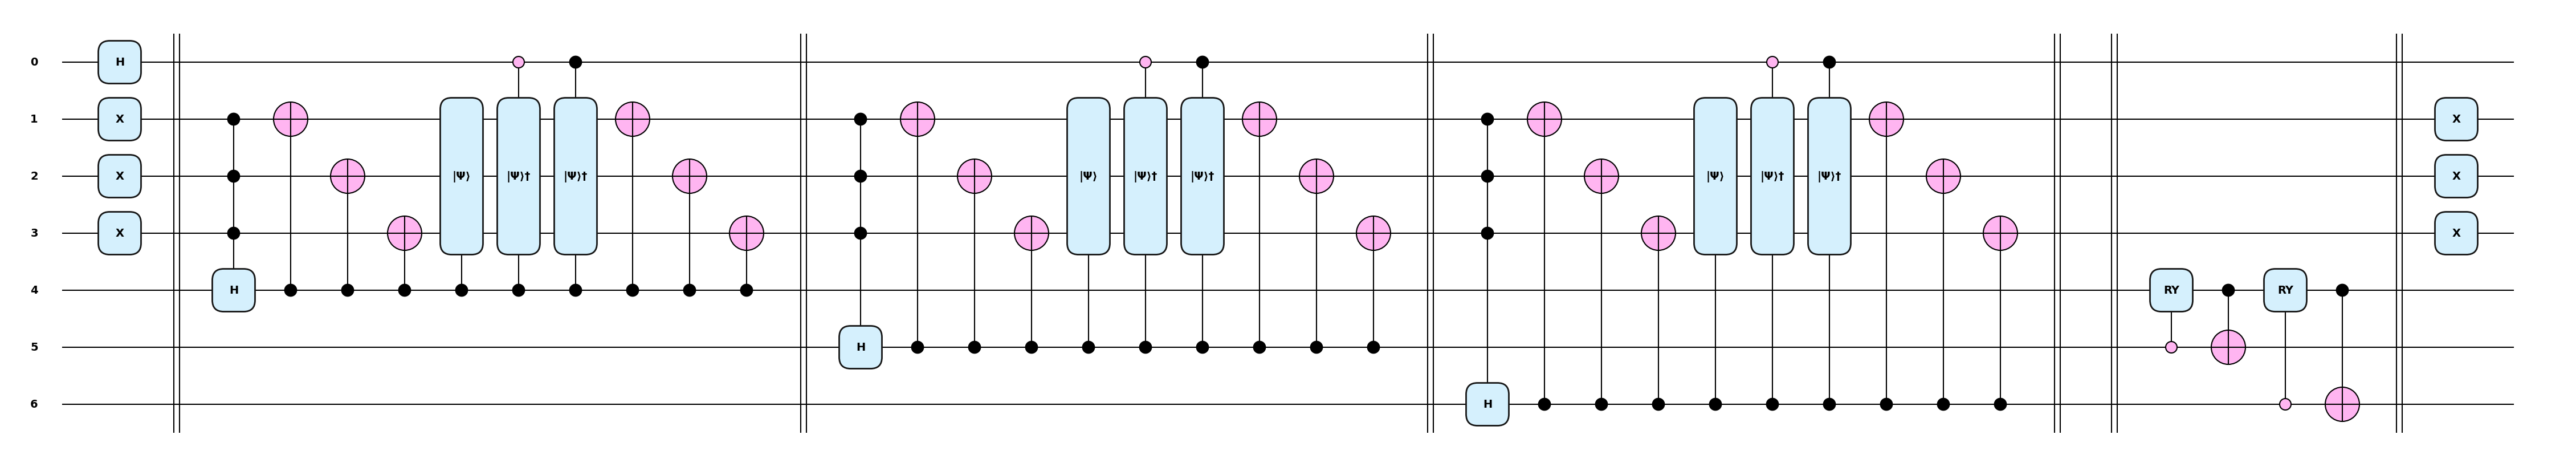
\includegraphics[scale=0.5, width=0.8\textwidth]{figs/theorem2_circuit_12110900.png}\
\caption{Theroem2의 quantum circuit 구조}
\label{fig:Theroem2-cricuit}
\end{figure}

이러한 회로와 MLP의 출력을 같은 $w , x, b$이 주어졌을 떄 동일한 결과를 나타내는지 확인하였다. 이때 output이 2차원이므로 이를 x,y평면에서 그래프로 나타내었으며 다음그래프를 보면 테일러 급수 d 차수가 늘어날 수록 비슷한 그래프가 되는 것을 볼 수 있다.

\begin{figure}[h]
    \centering
        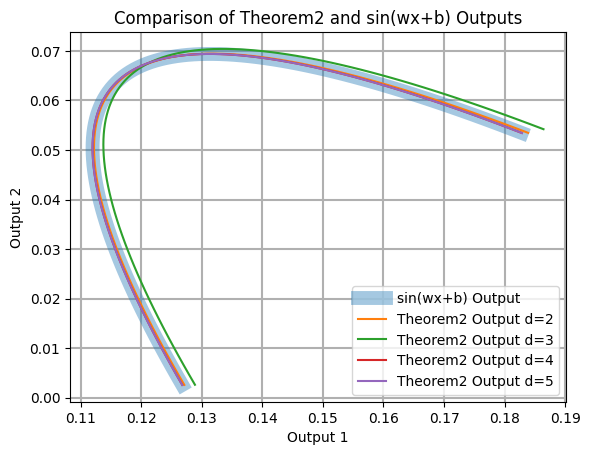
\includegraphics[scale=0.5, width=0.8\textwidth]{figs/output_theorem2_1211.png}\
\caption{sin(wx+b)를 ml과 qml로 나타낸 그래프이다.}
\label{fig:Theroem2-Experiment}
\end{figure}
